%==============================================================
%  OG-UPCR — Written Report
%  Paper: Unsupervised RGB-D Point Cloud Registration for Scenes
%         with Low Overlap and Photometric Inconsistency (ICCV 2025)
%
%  HOW TO COMPILE (Overleaf or local):
%   Requires LuaLaTeX (for Vietnamese Unicode text on the cover page).
%   latexmk   — latexmk -pdflua -interaction=nonstopmode -outdir=build report.tex
%==============================================================
\documentclass[11pt,a4paper]{article}

% ---- Layout -------------------------------------------------
\usepackage[top=1in,bottom=1in,left=1.1in,right=1.1in]{geometry}
\usepackage{setspace}
\setstretch{1.15}

% ---- Core packages ------------------------------------------
\usepackage{fontspec}
\setmainfont{lmroman10}[
  Extension = .otf,
  UprightFont = *-regular,
  BoldFont = *-bold,
  ItalicFont = *-italic,
  BoldItalicFont = *-bolditalic,
]
\usepackage{amsmath,amssymb}
\usepackage{booktabs}
\usepackage{multirow}
\usepackage{graphicx}
\graphicspath{{imgs/}{./imgs/}}
\usepackage{xcolor}
\usepackage{hyperref}
\usepackage{caption}
\usepackage{subcaption}
\usepackage{tikz}
\usetikzlibrary{arrows.meta, positioning, shapes.geometric}
\usepackage{enumitem}
\usepackage{parskip}

% ---- Colors (mirrored from slides.tex) ----------------------
\definecolor{ProbRed}{HTML}{C0392B}
\definecolor{OkGreen}{HTML}{1E8449}
\definecolor{AccentBlue}{HTML}{2C6FBB}
\definecolor{OrangeYellow}{HTML}{D4890B}
\definecolor{Purple}{HTML}{8E44AD}

% ---- TikZ styles --------------------------------------------
\tikzset{
  box/.style={rectangle, rounded corners, draw=#1, thick, fill=#1!10,
              minimum width=2.4cm, minimum height=0.7cm,
              font=\small, align=center},
  box/.default=AccentBlue,
  arr/.style={-{Stealth[length=2mm]}, thick},
}

% ---- Hyperref setup -----------------------------------------
\hypersetup{
  colorlinks=true,
  linkcolor=AccentBlue,
  citecolor=AccentBlue,
  urlcolor=AccentBlue,
}

% ---- Title (metadata only; cover page below is custom) -------
\title{Unsupervised RGB-D Point Cloud Registration for Scenes with Low Overlap and Photometric Inconsistency (OG-UPCR)}
\author{Nguyen Tat Chung}
\date{\today}

\begin{document}

%==============================================================
% Trang bìa (theo mẫu Trường Đại học Phenikaa)
%==============================================================
\begin{titlepage}
\thispagestyle{empty}
\setlength{\fboxsep}{1cm}
\setlength{\fboxrule}{0.6pt}
\noindent\fbox{%
  \begin{minipage}[c][\dimexpr\textheight-2\fboxsep-2\fboxrule\relax][c]{\dimexpr\textwidth-2\fboxsep-2\fboxrule\relax}
  \begin{center}
    {\bfseries BỘ GIÁO DỤC VÀ ĐÀO TẠO}\\
    {\bfseries TRƯỜNG ĐẠI HỌC PHENIKAA}\\[2pt]
    \rule{3.5cm}{0.4pt}

    \vfill

    
\includegraphics[width=0.55\linewidth]{phenikaa-uni-symbol.png}

    \vfill

    {\LARGE\bfseries BÁO CÁO MÔN HỌC}

    \vspace{2.5em}

    {\Large\bfseries TÊN ĐỀ TÀI:}\\[0.8em]
    {\large\bfseries UNSUPERVISED RGB-D POINT CLOUD REGISTRATION\\
    FOR SCENES WITH LOW OVERLAP\\
    AND PHOTOMETRIC INCONSISTENCY}\\[0.4em]
    {\normalsize\itshape (OG-UPCR, ICCV 2025)}\\[0.6em]
    {\normalsize\itshape Đăng ký đám mây điểm RGB-D không giám sát cho cảnh có\\
    độ chồng lấn thấp và không nhất quán quang trắc}

    \vfill

    \begin{tabular}{@{}l@{}}
      Học phần: \quad Thị giác máy tính (Computer Vision)\\
      % Bậc đào tạo: \quad Cao học (Thạc sĩ)
    \end{tabular}

    \vspace{2em}

    \begin{tabular}{@{}ll@{}}
      Học viên thực hiện: & Nguyễn Tất Chung \\[0.3em]
      Giảng viên hướng dẫn: & TS. Nguyễn Văn Tới
    \end{tabular}

    \vfill

    {\bfseries Hà Nội, tháng 8 năm 2026}
  \end{center}
  \end{minipage}%
}
\end{titlepage}

%==============================================================
\begin{abstract}
Point cloud registration — the task of finding the rigid transformation that aligns
two 3D scans — is a cornerstone of 3D computer vision, with applications in
robotics, autonomous driving, and 3D reconstruction. Unsupervised RGB-D methods
have shown strong results, but they break down when the two frames share only a
small overlapping region (\emph{low overlap}) or when the same surface appears
photometrically different across views (\emph{photometric inconsistency}). This
report summarises OG-UPCR (ICCV 2025), which addresses both problems with two
novel modules: \textbf{OCID} (Overlapping Constraint for Inliers Detection) uses a
global overlap ratio to reliably identify true inlier correspondences, and
\textbf{GRPA} (Gaussian Rendering for Photometric Adaptation) replaces the
conventional nearest-point rasterizer with 3D Gaussian splatting and learnable
per-pixel photometric adaptation. Trained end-to-end without ground-truth poses,
OG-UPCR achieves state-of-the-art unsupervised registration on ScanNet and the
challenging ScanNet1500 benchmark.
\end{abstract}

\tableofcontents
\newpage

%==============================================================
\section{Introduction and Problem Statement}
\label{sec:intro}
%==============================================================

\subsection{What is Point Cloud Registration?}

Point cloud registration is a \textbf{fundamental task in 3D vision}: given two
partial scans (frames) of a scene as sets of 3D points, the goal is to find the
rigid transformation that aligns them into a single, consistent coordinate system.

\begin{figure}[h]
  \centering
  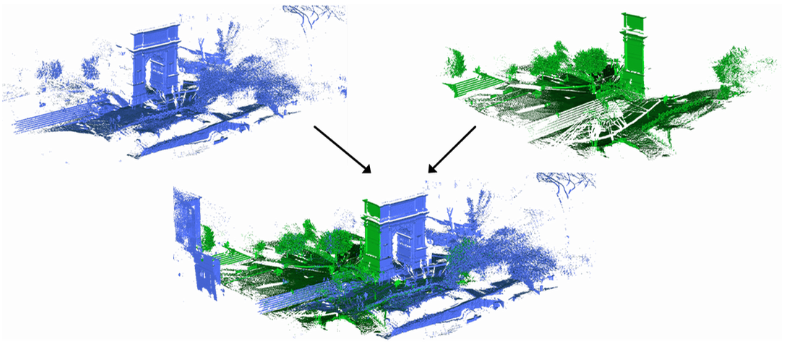
\includegraphics[width=0.72\linewidth]{imgs/1_what_is_pcr.png}
  \caption{Illustration of point cloud registration. Two partial scans $P$ and $Q$
  are aligned by estimating a rigid transformation $\mathbf{T}=\{\mathbf{R},\mathbf{t}\}$.}
  \label{fig:pcr}
\end{figure}

The typical pipeline (see Fig.~\ref{fig:pcr}) proceeds in three steps:
\begin{enumerate}[noitemsep]
  \item \textbf{Feature extraction} on both point clouds.
  \item \textbf{Correspondence estimation} — match features to produce point pairs.
  \item \textbf{Robust geometric fitting} — estimate the transformation from the correspondences.
\end{enumerate}

\subsection{Mathematical Definition}

Given two point clouds $P \in \mathbb{R}^{N\times 3}$ and $Q \in \mathbb{R}^{N\times 3}$,
find a transformation
\[
  \mathbf{T} = \{\mathbf{R}, \mathbf{t}\}, \qquad
  \mathbf{R}\in \mathrm{SO}(3),\quad \mathbf{t}\in\mathbb{R}^3
\]
that aligns the two scans.
The \textbf{correspondence set} obtained by feature matching is
\[
  C = \{\, \mathbf{p}_i, \mathbf{q}_j \mid \mathbf{p}_i \in P,\ \mathbf{q}_j \in Q \,\}.
\]
The optimal transformation minimises the alignment error:
\begin{equation}
  \underset{\mathbf{R},\mathbf{t}}{\arg\min}\ \sum_{i=1}^{n}
  \big\lVert \mathbf{R}\,\mathbf{p}_i + \mathbf{t} - \mathbf{q}_j \big\rVert_2^2
  \tag{1}
\end{equation}
where $n$ is the number of correspondences.

\subsection{Applications}

Registration underpins three broad application areas:
\begin{itemize}[noitemsep]
  \item \textbf{Navigation} — localization and mapping for robotics and autonomous driving.
  \item \textbf{Pose estimation} — recovering camera or object poses across frames.
  \item \textbf{3D reconstruction} — stitching partial scans into a complete 3D model.
\end{itemize}

\subsection{The Two Problems Addressed by OG-UPCR}
\label{sec:problems}

With cheap RGB-D sensors, unsupervised registration avoids the cost of ground-truth pose
collection. However, existing unsupervised methods assume that the geometric and photometric
information between the two frames is \emph{consistent} — an assumption that fails in many
real-world scenarios:

\begin{description}
  \item[\textcolor{ProbRed}{Low Overlap.}]
    The two frames share only a small common region. This produces many
    \textbf{correspondence outliers}, making feature identification and correspondence
    estimation unreliable. Inliers \emph{must} lie inside the overlapping region; outliers
    can therefore be filtered using an \textbf{overlapping constraint} — the key observation
    that motivates the OCID module.

  \item[\textcolor{ProbRed}{Photometric Inconsistency.}]
    The same surface appears different across frames due to reflections, lighting changes, or
    viewpoint variation. This breaks the feature-consistency assumption between the input
    frame and the rendered frame, hindering the model from learning \textbf{discriminative
    features} and causing the photometric loss to penalise correct poses.
\end{description}

%==============================================================
\section{Background and Related Work}
\label{sec:related}
%==============================================================

\subsection{Deep-Learning Descriptors for Registration}

Early \textbf{hand-crafted descriptors} (e.g.\ SIFT, FPFH) are sensitive to noise and not
robust to changes in point density. Modern \textbf{deep-learning descriptors} achieve much
better performance and split into two families:

\begin{itemize}[noitemsep]
  \item \textbf{Supervised methods} require ground-truth poses, limiting practical
    applicability and suffering domain gaps when transferred to new scenes.
  \item \textbf{Unsupervised methods} need no pose labels, making them attractive
    for real-world deployment. OG-UPCR belongs to this family.
\end{itemize}

Unsupervised methods further split by input type.

\paragraph{Geometric-based (point cloud only).}
\textbf{RIENet} performs reliable inlier evaluation via neighbourhood consensus.
\textbf{UDReg} learns the posterior distribution of Gaussian Mixture Models from point
clouds and predicts distribution-level correspondences. Their limitation: without texture
information, they struggle in \emph{geometrically weak regions} (floors, ceilings, walls)
and on repeated structures common in indoor scenes.

\paragraph{RGB-D based (point cloud + image).}
\textbf{LLT} uses a linear attention module to fuse geometric and texture features.
\textbf{PointMBF} introduces multi-scale bidirectional fusion of RGB-D information and
serves as the \emph{direct baseline} for OG-UPCR. Other methods in this family include
\textbf{UR\&R}, \textbf{BYOC}, and \textbf{CCAP}.

\subsection{The Standard Unsupervised RGB-D Pipeline and Its Failure Modes}
\label{sec:pipeline}

All prior unsupervised RGB-D methods share a common training framework built around a
\textbf{differentiable renderer} (typically PyTorch3D~\cite{ravi2020pytorch3d}). The
pipeline works as follows:

\begin{center}
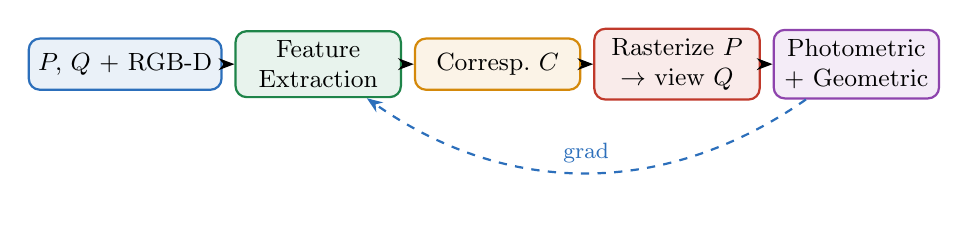
\begin{tikzpicture}[node distance=0.3cm and 0.15cm,
    box/.append style={minimum width=2.1cm, minimum height=0.65cm, font=\small}]
  \node[box=AccentBlue] (inp)  {$P,\,Q$ + RGB-D};
  \node[box=OkGreen, right=of inp] (feat) {Feature\\ Extraction};
  \node[box=OrangeYellow, right=of feat] (corr) {Corresp.\ $C$};
  \node[box=ProbRed, right=of corr] (rend) {Rasterize $P$\\ $\to$ view $Q$};
  \node[box=Purple, right=of rend] (loss) {Photometric\\ + Geometric};

  \draw[arr] (inp)  -- (feat);
  \draw[arr] (feat) -- (corr);
  \draw[arr] (corr) -- (rend);
  \draw[arr] (rend) -- (loss);
  \draw[arr, bend left=35, dashed, AccentBlue] (loss) to
    node[above, font=\footnotesize, midway] {grad} (feat);
\end{tikzpicture}
\end{center}

\textbf{Step 1 — Pose and rasterisation.} The current estimate $(\mathbf{R},\mathbf{t})$
is derived from $C$ via Weighted SVD; $P$ is transformed and projected into the image
space of $Q$ via intrinsics $\mathbf{K}_Q$:
\[
  (u_i,v_i,d_i) = \Pi_{\mathbf{K}_Q}(\mathbf{p}'_i),\quad
  \Pi_{\mathbf{K}}(\mathbf{x}) = \big(f_x\tfrac{x}{z}+c_x,\ f_y\tfrac{y}{z}+c_y,\ z\big).
\]
Each pixel takes the colour and depth of the \emph{nearest} 3D point.

\textbf{Step 2 — Consistency losses.}
\[
  L_{rgb} = \lVert I_{\text{rend}} - I_Q \rVert_1, \qquad
  L_{depth} = \lVert D_{\text{rend}} - D_Q \rVert_1.
\]

\textbf{Step 3 — Correspondence loss.}
\[
  L_{corr} = \frac{1}{|C|}\sum_{(\mathbf{p},\mathbf{q},w)\in C}
  w\, \lVert \mathbf{R}\mathbf{p} + \mathbf{t} - \mathbf{q} \rVert^2.
\]

\textbf{Step 4 — Total loss.}
$L = \lambda_{rgb}L_{rgb} + \lambda_{depth}L_{depth} + \lambda_{corr}L_{corr}$.

Because the renderer is \textbf{differentiable}, gradients of $L_{rgb}$ and $L_{depth}$
flow back through rasterisation into the feature encoders (KPConv, ResNet), so features
and pose are learned jointly \emph{without ground-truth poses}.

\textbf{Why this fails under low overlap and photometric inconsistency.}
Under \emph{low overlap}, $I_{\text{rend}}$ contains large empty regions that differ from
$I_Q$, making the losses misleading and producing many outlier correspondences.
Under \emph{photometric inconsistency}, the nearest-point rasteriser copies colours
directly, so $I_{\text{rend}} \neq I_Q$ even at the correct pose — penalising correct
transformations. Both pathologies stem from the same root cause: the PyTorch3D rasteriser
has \emph{no adaptive photometric modelling} and is fragile under viewpoint change.

\subsection{Correspondence Outlier Handling}

\textbf{RANSAC} and its variants are the standard for outlier-robust fitting, but they
are slow and require many iterations at high outlier rates.
\textbf{SC$^2$PCR} and \textbf{MAC} use \emph{second-order spatial compatibility} to
identify inliers more efficiently. However, they rely only on \emph{relative} spatial
constraints between correspondence pairs and ignore the global overlapping region. This
leaves many redundant pairs and reduces accuracy in low-overlap scenes.

\subsection{3D Gaussian Splatting (3DGS)}

3DGS~\cite{kerbl2023gaussiansplatting} represents a scene as a collection of 3D Gaussians
and renders them via differentiable alpha-compositing, producing smooth, view-dependent
images with strong gradients — superior to nearest-point rasterisation.
Related systems include \textbf{SplaTAM} (online SLAM with 3DGS, requires dense input),
\textbf{PixelSplat} (sparse-view radiance field), and \textbf{NoPoSplat} (PnP + 3DGS,
image-based, loses 3D information). OG-UPCR's GRPA module uses 3DGS from the
\emph{point-cloud perspective}, making it independent of the true pose and robust even
with sparse inputs.

%==============================================================
\section{Proposed Method — OG-UPCR}
\label{sec:method}
%==============================================================

OG-UPCR takes as input paired point clouds $P, Q$ together with their RGB-D frames
(following the PointMBF backbone) and produces a refined rigid transformation
$\mathbf{T}_{gs}^R$ through two novel modules: \textbf{OCID} and \textbf{GRPA}.
The full pipeline is illustrated in Fig.~\ref{fig:overview}.

\begin{figure}[h]
  \centering
  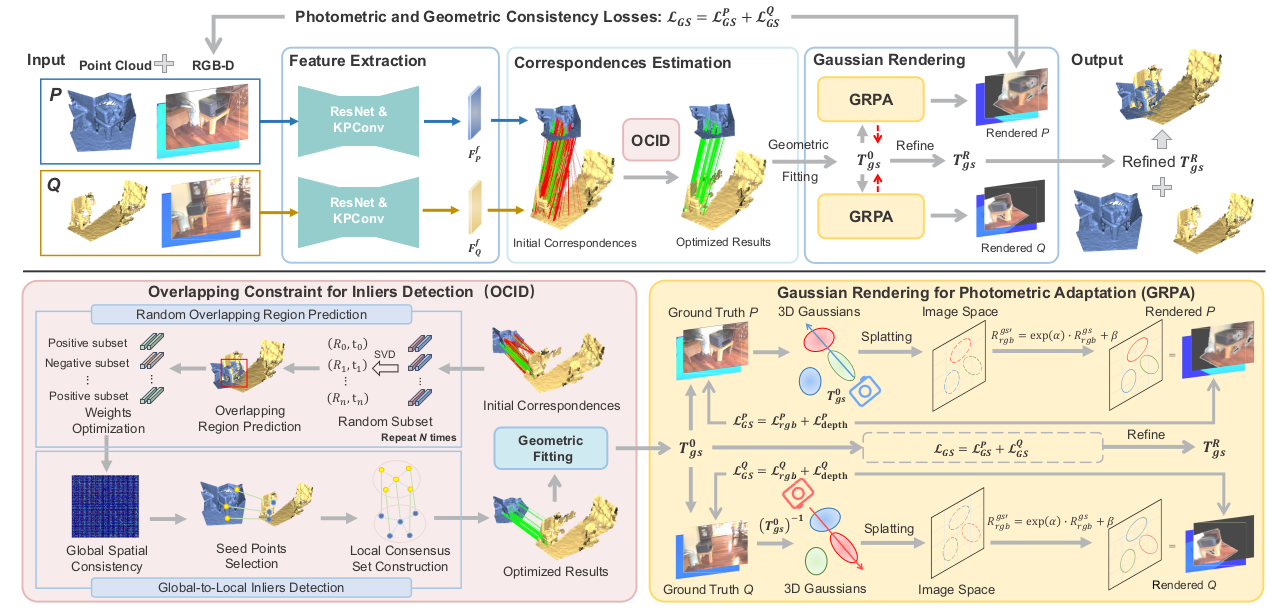
\includegraphics[width=\linewidth]{imgs/2_overview_OG-UPCR.png}
  \caption{Overview of OG-UPCR. Inputs: point clouds $P, Q$ plus their RGB-D frames.
  OCID produces a coarse transformation $\mathbf{T}_{gs}^0$; GRPA refines it to
  $\mathbf{T}_{gs}^R$. The entire system is trained end-to-end without ground-truth poses.}
  \label{fig:overview}
\end{figure}

\subsection{Feature Extraction}

\textbf{KPConv} extracts 3D geometric features from the point clouds; \textbf{ResNet}
extracts 2D image features from the RGB frames. A \emph{multi-scale bidirectional fusion}
module (inherited from PointMBF~\cite{zhang2023pointmbf}) cross-fuses the two streams at
multiple resolutions, producing fused descriptors
\[
  F_P^f,\; F_Q^f \in \mathbb{R}^{N\times C_{3D}}
\]
where each point carries both geometric and texture information.

\paragraph{Why bidirectional, multi-scale fusion?}
The two branches are exchanged in \emph{both} directions: image$\to$point gathers the
RGB feature at the pixel a 3D point projects to (using the depth map to establish the
pixel--point correspondence), while point$\to$image scatters each point's geometric
feature back onto the image plane to enrich the 2D stream. Earlier fusion schemes (e.g.\
LLT) exchange information in only one direction and typically at a single stage. Here,
this exchange happens at \emph{multiple} encoder--decoder resolutions, so the two
modalities reinforce each other from fine local detail up to coarse global context.
The payoff is complementary: texture cues disambiguate geometrically weak regions
(flat walls, floors, ceilings) where point-only descriptors are degenerate, while
geometric cues remain reliable in low-texture or poorly lit areas where image
descriptors are uninformative.

\subsection{Correspondence Estimation}
\label{sec:corresp}

For every point $\mathbf{p}_i \in P$, the nearest and second-nearest neighbours in feature
space are found in $F_Q^f$. \textbf{Lowe's ratio} measures match confidence:
\begin{equation}
  r_i = \frac{D(\mathbf{p}_i, \mathbf{q}_j^{1nn})}{D(\mathbf{p}_i, \mathbf{q}_j^{2nn})}
  \tag{2}
\end{equation}
A small $r_i$ signals a clear, unambiguous match; $r_i \to 1$ signals ambiguity
(feature non-discriminative).

\paragraph{Why a ratio, not a distance threshold?}
Lowe's original intuition (SIFT~\cite{lowe2004sift}) is that a correct match should be a
\emph{stand-out} candidate, not one of several equally-plausible options. The
\emph{absolute} distance to the nearest neighbour is not sufficient on its own: in
repetitive, low-texture regions (flat walls, floors, periodic patterns) many points share
similar features, so even an incorrect match can have a small absolute distance, while a
correct match in a difficult region can have a comparatively larger one. Comparing against
the \emph{second}-nearest neighbour instead measures \emph{uniqueness} — precisely what
determines whether a match can be trusted. Consequently $r_i \to 1$ is most common in
exactly these repetitive indoor structures, which is where unsupervised RGB-D methods are
most prone to outlier correspondences.

Rather than applying a hard cut-off as in classical SIFT matching (e.g.\ rejecting
$r>0.8$), OG-UPCR converts the ratio into a \emph{soft} confidence weight
$w = 1-r$, which is carried forward through the entire pipeline: it seeds the initial
correspondence set below, weights the Weighted SVD step inside OCID
(Sec.~\ref{sec:ocid}), and — after reward/penalty rescaling — determines seed selection
in Global-to-Local inlier detection and the per-pair weighting of $L_{corr}$
(Eq.~21). The correspondence weight is thus $w = 1 - r$. The top-$k$ matches
are retained in each direction ($P\to Q$ and $Q\to P$), giving the initial set:
\begin{equation}
  C_{\text{initial}} = \{(\mathbf{p}, \mathbf{q}, w)_m : 0 \le m < 2k\}
  \tag{3}
\end{equation}
$C_{\text{initial}}$ still contains many outliers; OCID filters them.

\subsection{OCID: Overlapping Constraint for Inliers Detection}
\label{sec:ocid}

OCID produces a reliable, well-distributed inlier set $C_f$ and a coarse transformation
$\mathbf{T}_{gs}^0$. It has two components.

\subsubsection{(a) Random Overlapping Region Prediction}

Inspired by RANSAC, this component iteratively assigns reward/penalty weights based on
whether a random subset of correspondences supports a pose with sufficient overlap.

\begin{enumerate}[noitemsep]
  \item Sample a random subset $C_n$ (fraction $r=0.2$) from $C_{\text{initial}}$;
    apply \textbf{Weighted SVD} to obtain a candidate pose $\mathbf{T}_s$.
  \item Transform $P' = \mathbf{T}_s \odot P$ and measure the \textbf{overlap ratio}:
    \begin{equation}
      O_p = \frac{1}{N}\sum_{n=1}^{N_{P'}}
      \bigl[\!\bigl[\,\lVert \mathbf{p}'_n - \mathbf{q}_n\rVert < \tau\,\bigr]\!\bigr],
      \qquad \tau = 5\,\text{cm}
      \tag{6}
    \end{equation}
  \item If $O_p \ge O_{thr}$, the subset is mostly inliers (\emph{positive}): reward with
    weight $w_r > 1$.  Otherwise, it is mostly outliers (\emph{negative}): penalise with
    $w_p < 1$.  The constraint $w_r \cdot w_p = 1$ stabilises the weights across
    iterations.
    \begin{equation}
      w_r \cdot w_p = 1
      \tag{7}
    \end{equation}
  \item Repeat $N$ times. True inliers accumulate reward; outliers accumulate penalty.
    The top-$k$ correspondences by final weight form the optimised set:
    \begin{equation}
      C_f = \bigl\{(\mathbf{p}, \mathbf{q}, w)_f : 0 \le m < 2k_f\bigr\}
      \tag{8}
    \end{equation}
\end{enumerate}

\subsubsection{(b) Global-to-Local Inliers Detection}

Even after step (a), inliers may cluster in a small spatial region, which destabilises
geometric fitting. This component promotes uniform spatial coverage.

\textbf{Second-order spatial compatibility (SC$^2$)} is computed globally over $C_f$:
\begin{equation}
  SC^2_{ij} = C_{ij}\cdot \sum_{k=1}^{N} C_{ik}\,C_{kj}
  \tag{9}
\end{equation}
\begin{equation}
  C_{ij} =
  \begin{cases}
    1, & \bigl|\,\lVert\mathbf{p}_i-\mathbf{p}_j\rVert
         - \lVert\mathbf{q}_i-\mathbf{q}_j\rVert\,\bigr| \le d_{thr}\\
    0, & \text{otherwise}
  \end{cases}
  \quad (d_{thr} = 10\,\text{cm})
  \tag{10}
\end{equation}
\begin{equation}
  d_{ij} = \lVert\mathbf{p}_i - \mathbf{p}_j\rVert_2 - \lVert\mathbf{q}_i - \mathbf{q}_j\rVert_2
  \tag{11}
\end{equation}

Seed points are selected greedily: the point with the highest $SC^2$ score in a radius
$R$ neighbourhood is chosen, ensuring seeds are \emph{spatially spread} over the
overlapping region. Each seed and its $K$ nearest neighbours form a \textbf{consensus
set}. Weighted SVD is applied to each consensus set; the one with the most inliers
(below a distance threshold) yields the coarse transformation $\mathbf{T}_{gs}^0$.

\subsubsection{OCID Pipeline Summary}

\begin{center}
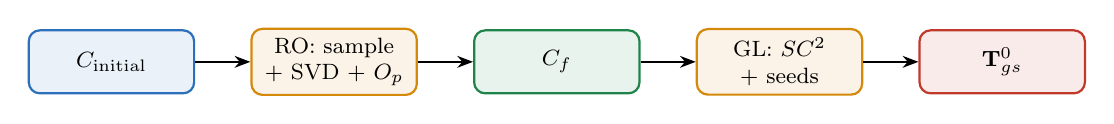
\begin{tikzpicture}[node distance=0.5cm and 0.7cm,
    box/.append style={minimum width=2.1cm, minimum height=0.8cm, font=\footnotesize}]
  \node[box=AccentBlue] (init) {$C_{\text{initial}}$};
  \node[box=OrangeYellow, right=of init] (ro) {RO: sample\\ + SVD + $O_p$};
  \node[box=OkGreen, right=of ro] (cf) {$C_f$};
  \node[box=OrangeYellow, right=of cf] (gl) {GL: $SC^2$\\ + seeds};
  \node[box=ProbRed, right=of gl] (t0) {$\mathbf{T}_{gs}^0$};

  \draw[arr] (init) -- (ro);
  \draw[arr] (ro)   -- (cf);
  \draw[arr] (cf)   -- (gl);
  \draw[arr] (gl)   -- (t0);
\end{tikzpicture}
\end{center}
Correspondences flow left to right: RO selects the top-$k_f$ correspondences by
reward/penalty weight to form $C_f$; GL then selects the pose from the consensus set
with the most inliers to obtain $\mathbf{T}_{gs}^0$.

\paragraph{How OCID differs from RANSAC and SC$^2$-PCR/MAC.} Classical RANSAC evaluates
random subsets purely by their inlier count under a pairwise distance threshold, which is
slow to converge under high outlier ratios. SC$^2$-PCR and MAC instead rely on
\emph{relative} spatial-compatibility constraints between correspondence pairs
(Sec.~\ref{sec:related}), but never check whether a candidate pose is consistent with the
scene as a whole. OCID's key departure is to score candidate poses with a \emph{global
overlapping-region constraint} (the overlap ratio $O_p$, Eq.~6): a true inlier must lie
inside the region where $P$ and $Q$ actually overlap, which is a much stronger and more
direct signal than pairwise distance preservation alone. This lets OCID reject outliers
effectively even under low overlap, while the subsequent Global-to-Local step keeps the
computational cost bounded by only refining within the already-filtered set $C_f$, rather
than the full pairwise compatibility matrix over $C_{\text{initial}}$.

\subsection{GRPA: Gaussian Rendering for Photometric Adaptation}
\label{sec:grpa}

GRPA refines the coarse $\mathbf{T}_{gs}^0$ into the final $\mathbf{T}_{gs}^R$ while
adapting to photometric inconsistency. It replaces the PyTorch3D rasteriser with
3D Gaussian splatting.

\textbf{Point $\to$ 3D Gaussian.} Each 3D point is lifted to a Gaussian with position
$\mu_{3D}$, colour $\mathbf{c} \in \mathbb{R}^3$, radius $r$, and opacity $o \in [0,1]$:
\begin{equation}
  g(\mathbf{x}) = o\,\exp\!\Bigl(-\frac{\lVert \mathbf{x}-\mu_{3D}\rVert^2}{2 r_{3D}^2}\Bigr)
  \tag{12}
\end{equation}

\textbf{Alpha-blended rasterisation.} Each pixel $\rho$ in the rendered image accumulates
contributions from the $n$ Gaussians sorted by depth:
\begin{equation}
  R^{gs}_{rgb}(\mathbb{G},\mathbf{T}) =
  \sum_{i=1}^{n} c_i\,g_i(\rho)\prod_{j=1}^{i-1}\bigl(1 - g_j(\rho)\bigr)
  \tag{13}
\end{equation}
The 2D projection follows $\mu_{2D} = \mathbf{K}\mathbf{T}\,\mu_{3D}/d$, $r_{2D} = f/d$
(Eq.~14). $\mathbf{T}\mu_{3D}$ maps the point from world to camera coordinates using the
extrinsic $\mathbf{T}=[\mathbf{R}\,|\,\mathbf{t}]$ — the very pose OG-UPCR is trying to
refine — while dividing by depth $d$ produces the familiar perspective effect. Because
this projection is non-linear, projecting a Gaussian's full covariance $\Sigma_{3D}$ (not
just its centre) in general 3DGS requires a local linear approximation via the projection
Jacobian $\mathbf{J}$, $\Sigma_{2D} = \mathbf{J}\mathbf{W}\Sigma_{3D}\mathbf{W}^\top
\mathbf{J}^\top$ (EWA splatting~\cite{kerbl2023gaussiansplatting}); OG-UPCR uses
\emph{isotropic} Gaussians (a single scalar radius $r_{3D}$ rather than a full covariance),
so this reduces to the simple scalar relation $r_{2D}=f\,r_{3D}/d$ used above.

\textbf{Per-pixel photometric adaptation.} Learnable parameters $\alpha$ and $\beta$
correct gain and bias per pixel:
\begin{equation}
  R^{gs'}_{rgb} = \exp(\alpha)\cdot R^{gs}_{rgb} + \beta
  \tag{15}
\end{equation}
An analogous rendered depth image is obtained:
\begin{equation}
  R^{gs}_{depth}(\mathbb{G},\mathbf{T}) =
  \sum_{i=1}^{n} d_i\,g_i(\rho_a)\prod_{j=1}^{i-1}\bigl(1 - g_j(\rho_a)\bigr)
  \tag{16}
\end{equation}

\paragraph{Why $\exp(\alpha)$ controls contrast and $\beta$ controls brightness.} Eq.~15 is
an affine map $R'=aR+b$ with gain $a=\exp(\alpha)$ and bias $b=\beta$, applied
independently per pixel. Writing brightness as the mean intensity and contrast as the
intensity spread (standard deviation), the affine transform gives
$\mathrm{mean}(aR+b)=a\,\mathrm{mean}(R)+b$ but
$\mathrm{std}(aR+b)=a\,\mathrm{std}(R)$ — the additive term $b$ cancels when
differencing two pixel values, $(ax_1+b)-(ax_2+b)=a(x_1-x_2)$, so it leaves relative
intensity gaps (contrast) untouched and only shifts the overall level (brightness).
The gain is parameterised as $\exp(\alpha)$ rather than a raw scalar for two reasons:
it is guaranteed positive for any $\alpha\in\mathbb{R}$ (a negative multiplicative gain
is physically meaningless), and optimising in log-space keeps the gradient symmetric
around the neutral initialisation $\alpha=0$ (i.e.\ gain $=1$), since doubling versus
halving brightness correspond to $\pm\ln 2$ shifts in $\alpha$. Physically, sensor
irradiance is well approximated by $I_{\text{obs}}\approx g\cdot I_{\text{scene}}+o$,
where gain $g$ absorbs exposure/ISO/white-balance differences and offset $o$ absorbs
ambient/indirect lighting and sensor black level; $\exp(\alpha)R+\beta$ is precisely the
inverse of this model, so $(\alpha,\beta)$ can absorb the two most common sources of
cross-frame photometric mismatch. Crucially, $(\alpha,\beta)$ are \emph{per-pixel} and
\emph{re-optimised for every frame pair} (see below), not fixed network weights — they
give the photometric loss an outlet for lighting differences so that the remaining
residual reflects geometric (pose) error rather than illumination, preventing gradients
from incorrectly pulling $\mathbf{T}$ toward a pose that merely happens to match the
wrong lighting.

\textbf{Rendering loss.} For point cloud $P$, the rendering loss is:
\begin{equation}
  L^P_{gs} = L^P_{rgb} + L^P_{depth}
  \tag{17}
\end{equation}
\begin{equation}
  L^P_{rgb} = \bigl\lVert R^{gs'}_{rgb}(\mathbb{G}^Q, \mathbf{T}^0_{gs}) - I^P \bigr\rVert_1
  \tag{18}
\end{equation}
\begin{equation}
  L^P_{depth} = \bigl\lVert R^{gs}_{depth}(\mathbb{G}^Q, \mathbf{T}^0_{gs}) - D^P \bigr\rVert_1
  \tag{19}
\end{equation}
where $\mathbb{G}^Q$ are Gaussians associated with $Q$, and $I^P$, $D^P$ are the true
RGB image and depth of frame $P$. The camera extrinsic is set to the identity matrix
$\mathbf{T}_0$, making the render \emph{independent of the true pose}; the coarse
$\mathbf{T}_{gs}^0$ is iteratively refined into $\mathbf{T}_{gs}^R$ by minimising
$L_{gs}$. An analogous $L^Q_{gs}$ is computed for $Q$.

\paragraph{Cross-view rendering and GRPA's dual role.} Concretely, GRPA renders
\emph{across} the two views: the Gaussians built from $Q$ are placed at extrinsic
$\mathbf{T}_{gs}^0$ and rendered from the reference viewpoint $\mathbf{T}_0$, then
compared against the \emph{real} image and depth of $P$ (Eq.~18--19), and symmetrically
for $Q$. Because this optimisation needs only the input RGB-D frames — no ground-truth
pose — it can run identically at two different stages of the pipeline: during
\emph{training}, gradients from $L_{gs}$ flow back through the differentiable Gaussian
renderer into the KPConv/ResNet backbone, jointly shaping the learned features; at
\emph{inference}, with the backbone weights frozen, the same minimisation is re-run for
each individual test pair to refine its own $\mathbf{T}_{gs}^0$ and $(\alpha,\beta)$ into
$\mathbf{T}_{gs}^R$ via a handful of gradient steps. GRPA is therefore not merely a
training-time loss — it doubles as a test-time pose-refinement procedure specific to
every frame pair it sees.

\textbf{Why GRPA is superior to PyTorch3D rasterisation:}
\begin{enumerate}[noitemsep]
  \item \emph{Soft rendering}: alpha-blending produces smooth, continuous images and
    stronger gradients than the hard nearest-point assignment.
  \item \emph{Photometric adaptation}: the learnable $(\alpha, \beta)$ per pixel absorbs
    gain/bias shifts from lighting or reflectance changes, so the photometric loss no
    longer penalises correct poses.
  \item \emph{Sparse-input robustness}: the finite Gaussian radius fills gaps in the
    rendered image that would otherwise appear as empty pixels under low overlap.
\end{enumerate}

\subsection{Loss Function}
\label{sec:loss}

The total training loss is unsupervised — no ground-truth poses are needed:
\begin{equation}
  L = \lambda_{gs}\, L_{gs} + \lambda_{corr}\, L_{corr}
  \tag{20}
\end{equation}
where $L_{gs} = L^P_{gs} + L^Q_{gs}$ is the photometric-and-depth consistency loss from
GRPA, and $L_{corr}$ is the correspondence consistency loss on the OCID-filtered set $C_f$:
\begin{equation}
  L_{corr} = \sum_{(\mathbf{p},\mathbf{q},w)_f \in C_f}
  w_f\,\bigl(\mathbf{T}_{gs}^R \odot \mathbf{p}_f - \mathbf{q}_f\bigr)^2 \big/ 2k_f
  \tag{21}
\end{equation}
$L_{gs}$ provides global photometric and geometric supervision through differentiable
rendering; $L_{corr}$ provides direct geometric supervision on reliable correspondences.
Together they form a closed self-supervised loop: better features $\to$ better
correspondences $\to$ better poses $\to$ better features.

\subsection{Training and Inference Procedure}
\label{sec:training}

Minimising $L$ in Eq.~20 does not target zero loss; it involves \textbf{two nested
optimisation loops} with different scopes, different variables, and different stopping
criteria, summarised in Table~\ref{tab:loops}.

\textbf{Outer loop — backbone training.} For each training pair: (1) \emph{forward} —
extract features, form correspondences, run OCID to obtain $\mathbf{T}_{gs}^0$, run GRPA
rendering, and evaluate $L$; (2) \emph{backward} — gradients flow through the
differentiable Gaussian renderer back into the KPConv/ResNet backbone; (3) an optimiser
(e.g.\ Adam) updates the backbone weights. Training stops either after a fixed number of
epochs, or when validation-set registration metrics (rotation/translation error, chamfer
distance) plateau, with the best-performing checkpoint retained (early stopping).

\textbf{Inner loop — GRPA refinement at inference.} With the backbone frozen, GRPA
re-runs the same rendering-loss minimisation for a \emph{single} test pair, refining only
$\mathbf{T}$ and $(\alpha,\beta)$ over a handful of gradient steps
($\mathbf{T}_{gs}^0 \to \mathbf{T}_{gs}^R$), stopping after a fixed step budget or once the
pose change between steps falls below a threshold. No ground truth is required, so this
runs identically at test time.

\begin{table}[h]
\centering
\caption{The two nested optimisation loops in OG-UPCR.}
\label{tab:loops}
\resizebox{\linewidth}{!}{%
\begin{tabular}{lccc}
\toprule
Loop & Optimises & Data scope & Stopping criterion \\
\midrule
Outer (training) & Backbone weights & Full training set & Fixed epochs / validation plateau \\
Inner (GRPA, inference) & $\mathbf{T}$, $\alpha,\beta$ & One frame pair & Fixed steps / pose convergence \\
\bottomrule
\end{tabular}
}
\end{table}

\textbf{Why the loss never reaches zero.} An irreducible residual always remains: regions
of $P$ and $Q$ that do not overlap cannot be matched by rendering; sensor noise,
occlusion, and depth errors add further error; and $(\alpha,\beta)$ are only an affine
correction, so some non-linear photometric effects are never fully absorbed. The
practical objective is therefore not "loss $\to 0$" but training until the learned
features are discriminative enough to yield accurate correspondences and poses — judged
by validation registration accuracy, not by the raw loss value.

%==============================================================
\section{Experiments and Results}
\label{sec:experiments}
%==============================================================

\subsection{Experimental Settings}

\paragraph{Datasets.}
Following PointMBF~\cite{zhang2023pointmbf}, OG-UPCR is evaluated on three real-world
indoor datasets:
\begin{itemize}[noitemsep]
  \item \textbf{3DMatch} — 122k / 1.5k / 1.5k view pairs for train / val / test.
  \item \textbf{ScanNet} — 1594k / 12.6k / 26k view pairs for train / val / test.
  \item \textbf{ScanNet1500} — 1500 test pairs with an average interval of 480.8 frames,
    featuring \emph{low overlap and large viewpoint variation}; the most challenging benchmark.
\end{itemize}

\paragraph{Metrics.}
Registration accuracy and error are measured on three axes:
\textbf{rotation error} (degrees), \textbf{translation error} (cm), and
\textbf{chamfer distance} (mm). For each axis both accuracy at fixed thresholds and
mean/median error are reported, following the evaluation protocol introduced by
UR\&R~\cite{elbanani2021urr} and adopted by PointMBF for ScanNet/ScanNet1500, which
allows direct, fair comparison against all baselines.

Within the Rotation and Translation groups, the result tables (Tables~\ref{tab:scannet}
and~\ref{tab:scannet1500}) report five columns each, split into two distinct kinds of
statistic:

\begin{itemize}[noitemsep]
  \item \textbf{Three accuracy columns} (e.g.\ ``5, 10, 45'' for rotation in degrees, or
    ``5, 10, 25'' for translation in cm) report the \emph{percentage of test pairs} whose
    error falls below the stated physical threshold:
    \begin{equation}
      \mathrm{Acc@}\theta = \frac{1}{|\mathcal{D}|}\sum_{i=1}^{|\mathcal{D}|}
      \bigl[\!\bigl[\, e_i < \theta \,\bigr]\!\bigr] \times 100\%
      \tag{22}
    \end{equation}
    Higher is better. The header value ($5$, $10$, $45$, \ldots) is the threshold in
    physical units (degrees or cm), \emph{not} a percentage — only the reported cell
    value is a percentage.
  \item \textbf{Mean and Med(ian)} report the aggregate \emph{error itself} (in degrees
    or cm) over the whole test set, not a percentage. Mean is sensitive to outliers — a
    handful of severe failures can dominate it — while the median is robust and reflects
    the error of a "typical" pair. Lower is better for both; a large Mean/Med gap signals
    a long tail of hard failures.
\end{itemize}

\textbf{Chamfer distance} complements these pose-space metrics with a direct,
correspondence-free measure of geometric alignment quality: after applying the estimated
transformation $\mathbf{T}$ to $P$ (giving $X$) and letting $Y=Q$,
\begin{equation}
  \mathrm{CD}(X,Y) = \frac{1}{|X|}\sum_{\mathbf{x}\in X}\min_{\mathbf{y}\in Y}
  \lVert \mathbf{x}-\mathbf{y}\rVert^2 \;+\;
  \frac{1}{|Y|}\sum_{\mathbf{y}\in Y}\min_{\mathbf{x}\in X}\lVert \mathbf{y}-\mathbf{x}\rVert^2
  \tag{23}
\end{equation}
i.e.\ the average nearest-neighbour distance in \emph{both} directions, which is
symmetric and penalises both missing and spurious overlap without requiring known point
correspondences. It captures cases where rotation/translation error alone may not fully
reflect how well the two surfaces actually align in 3D space. As with rotation and
translation error, lower chamfer distance is better, while the accompanying accuracy
columns (e.g.\ ``$<1$mm'') again report the percentage of pairs below threshold.

\paragraph{Competitors.}
Three groups:
\begin{itemize}[noitemsep]
  \item \textbf{Conventional}: SIFT, SuperPoint, FCGF.
  \item \textbf{Supervised} (trained with ground-truth poses): 3DMVReg, REGTR, BUFFER,
    PARENet.
  \item \textbf{Unsupervised}: UR\&R, BYOC, LLT, PointMBF (baseline), CCAP.
\end{itemize}
For supervised methods, generalisation is evaluated by using models trained on 3DMatch
and testing on ScanNet.

\subsection{Evaluation on ScanNet}

Table~\ref{tab:scannet} reproduces the main quantitative results on ScanNet. Trained on
3DMatch, OG-UPCR achieves \textbf{state-of-the-art} performance among all unsupervised
methods and outperforms all supervised methods on most metrics — demonstrating excellent
generalisation to unseen scenes. Trained on ScanNet, the baseline is nearly saturated,
yet OG-UPCR still achieves average reductions in rotation/translation/chamfer errors of
\textbf{40.0\% / 34.5\% / 41.3\%} compared to the strongest prior unsupervised method.

\begin{table}[h]
\centering
\caption{Pairwise registration on ScanNet. Best unsupervised result in \textbf{bold};
  second-best \underline{underlined}. ``Pose Sup'' = trained with ground-truth poses.
  Accuracy values are percentages; error values are mean/median.}
\label{tab:scannet}
\resizebox{\linewidth}{!}{%
\begin{tabular}{llc ccc cc ccc cc ccc cc c}
\toprule
\multirow{2}{*}{Method} & \multirow{2}{*}{Train} & \multirow{2}{*}{Pose Sup}
  & \multicolumn{5}{c}{Rotation ($^\circ$)}
  & \multicolumn{5}{c}{Translation (cm)}
  & \multicolumn{5}{c}{Chamfer (mm)}
  & \multirow{2}{*}{Time (s)} \\
\cmidrule(lr){4-8}\cmidrule(lr){9-13}\cmidrule(lr){14-18}
 & & & 5 & 10 & 45 & Mean & Med
       & 5 & 10 & 25 & Mean & Med
       & 1 & 5 & 10 & Mean & Med & \\
\midrule
SIFT        & --        &   & 55.2 & 75.7 & 89.2 & 17.7 & 44.3 & 17.7 & 44.5 & 79.8 & 26.5 & 11.2 & 38.1 & 70.6 & 78.3 & 42.6 & 1.7 & -- \\
SuperPoint  & --        &   & 65.5 & 86.9 & 96.6 & 8.9  & 3.5  & 21.2 & 51.7 & 88.0 & 16.1 & 9.7  & 45.7 & 81.1 & 88.2 & 19.2 & 1.2 & -- \\
FCGF        & --        & \checkmark & 70.2 & 87.7 & 96.2 & 9.3  & 5.3  & 27.5 & 58.3 & 82.9 & 23.6 & 8.3  & 52.0 & 78.0 & 83.7 & 24.4 & 0.9 & 0.129 \\
\midrule
3DMVReg     & 3DMatch   & \checkmark & 87.7 & 93.2 & 97.0 & 6.0  & 1.2  & 69.0 & 83.1 & 91.8 & 11.7 & 2.9  & 78.9 & 89.2 & 91.8 & 10.2 & \underline{0.2} & -- \\
REGTR       & 3DMatch   & \checkmark & 89.0 & 93.9 & 98.6 & 4.4  & 1.6  & 61.4 & 80.4 & 93.2 & 13.5 & 3.8  & 79.0 & 91.3 & 93.6 & 13.5 & \underline{0.2} & -- \\
BUFFER      & 3DMatch   & \checkmark & 95.9 & 98.4 & 99.5 & 2.4  & 0.9  & 79.6 & 92.3 & 96.9 & 5.7  & 2.4  & 93.6 & 97.5 & 98.6 & 4.2  & \textbf{0.2} & -- \\
PARENet     & 3DMatch   & \checkmark & 97.5 & 98.3 & \underline{99.5} & 1.9  & 0.7  & 85.9 & 95.7 & 97.0 & 3.9  & 1.8  & 94.2 & 97.9 & 98.6 & 4.2  & \underline{0.2} & 0.165 \\
\midrule
UR\&R       & 3DMatch   &   & 92.3 & 95.8 & 98.5 & 3.4  & 0.8  & 77.2 & 89.6 & 96.1 & 7.3  & 2.3  & 86.0 & 94.6 & 96.1 & 5.9  & \textbf{0.1} & 0.070 \\
UR\&R       & 3DMatch   &   & 87.6 & 93.1 & 98.3 & 4.3  & 1.0  & 69.2 & 84.0 & 93.8 & 9.5  & 2.8  & 79.7 & 91.3 & 94.0 & 7.2  & 0.2 & 0.071 \\
BYOC        & 3DMatch   &   & 66.5 & 87.0 & 97.8 & 7.4  & 4.5  & 30.7 & 57.6 & 88.7 & 18.6 & 8.2  & 58.4 & 82.9 & 88.5 & 9.5  & 0.9 & -- \\
LLT         & 3DMatch   &   & 93.4 & 96.5 & 98.8 & 2.5  & 0.8  & 76.9 & 90.2 & 96.7 & 5.5  & 2.2  & 86.4 & 95.1 & 96.8 & 4.6  & \textbf{0.1} & 0.125 \\
PointMBF    & 3DMatch   &   & 94.6 & 97.8 & \underline{99.5} & 3.0  & 0.8  & 81.0 & 92.0 & 97.1 & 6.2  & 2.1  & 91.4 & 96.8 & 97.4 & 4.9  & \textbf{0.1} & 0.079 \\
CCAP        & 3DMatch   &   & 95.6 & 98.1 & --   & 2.4  & 0.7  & 81.5 & 92.3 & --   & 3.7  & 1.9  & --   & --   & --   & --   & --  & -- \\
\textbf{Ours} & 3DMatch &   & \textbf{97.9} & \textbf{98.9} & \textbf{99.5} & \textbf{1.8} & \textbf{0.7} & \textbf{87.7} & \textbf{96.2} & \textbf{98.6} & \textbf{3.3} & \textbf{1.8} & \textbf{95.3} & \textbf{98.4} & \textbf{98.8} & \textbf{3.3} & \textbf{0.1} & 0.136 \\
\midrule
UR\&R       & ScanNet   &   & 92.7 & 95.8 & 98.5 & 3.4  & 0.8  & 77.2 & 89.6 & 96.1 & 7.3  & 2.3  & 86.0 & 94.6 & 96.1 & 5.9  & \textbf{0.1} & 0.071 \\
BYOC        & ScanNet   &   & 86.5 & 95.2 & 99.1 & 3.8  & 1.7  & 56.4 & 80.6 & 96.3 & 8.7  & 4.3  & 78.1 & 93.9 & 96.4 & 5.6  & 0.3 & -- \\
LLT         & ScanNet   &   & 95.5 & 97.6 & 99.3 & 2.1  & 0.8  & 80.4 & 92.2 & 97.8 & 5.8  & 2.3  & 84.1 & 96.8 & 97.6 & 4.6  & \textbf{0.1} & 0.125 \\
PointMBF    & ScanNet   &   & 96.0 & 97.6 & \underline{98.9} & 2.5  & 0.7  & 83.9 & 93.5 & 97.7 & 5.6  & \underline{1.9} & 92.8 & \underline{97.3} & 97.9 & 4.7  & \textbf{0.1} & 0.079 \\
CCAP        & ScanNet   &   & 97.1 & 98.2 & --   & 1.9  & --   & 85.9 & 93.6 & --   & --   & 1.8  & --   & --   & --   & --   & --  & -- \\
\textbf{Ours} & ScanNet &   & \textbf{98.3} & \textbf{99.2} & \textbf{99.7} & \textbf{1.5} & \textbf{0.7} & \textbf{88.8} & \textbf{96.7} & \textbf{99.0} & \textbf{3.3} & \textbf{1.7} & \textbf{96.1} & \textbf{98.8} & \textbf{99.1} & \textbf{2.8} & \textbf{0.1} & 0.136 \\
\bottomrule
\end{tabular}
}
\end{table}

\subsection{Evaluation on ScanNet1500}

ScanNet1500 is the most challenging benchmark: view pairs are sampled far apart (avg.
480.8 frames), resulting in low overlap and large viewpoint variation that defeat most
unsupervised methods. Table~\ref{tab:scannet1500} shows results.

OG-UPCR (trained on 3DMatch) is \emph{comparable to the supervised BUFFER} on the most
stringent thresholds and far above all other unsupervised methods. Trained on ScanNet,
it achieves the best registration results overall, with rotation accuracy $<5^\circ$ of
\textbf{81.3\%} and chamfer accuracy $<1\,$mm of \textbf{72.4\%}.

\begin{table}[h]
\centering
\caption{Pairwise registration on ScanNet1500. Best unsupervised in \textbf{bold}.
  OG-UPCR is comparable to the \emph{supervised} BUFFER and significantly outperforms
  all other unsupervised methods.}
\label{tab:scannet1500}
\resizebox{\linewidth}{!}{%
\begin{tabular}{llc ccc c ccc c ccc c}
\toprule
\multirow{2}{*}{Method} & \multirow{2}{*}{Train} & \multirow{2}{*}{Pose Sup}
  & \multicolumn{4}{c}{Rotation ($^\circ$)}
  & \multicolumn{4}{c}{Translation (cm)}
  & \multicolumn{4}{c}{Chamfer (mm)} \\
\cmidrule(lr){4-7}\cmidrule(lr){8-11}\cmidrule(lr){12-15}
 & & & 5 & 10 & 45 & Med
       & 5 & 10 & 25 & Med
       & 1 & 5 & 10 & Med \\
\midrule
LLT      & 3DMatch   &            & 36.1 & 49.9 & 79.9 & 10.0 & 17.2 & 29.9 & 46.6 & 29.6 & 23.5 & 40.4 & 48.3 & 12.1 \\
PointMBF & 3DMatch   &            & 51.1 & 60.8 & 82.8 & 4.7  & 31.5 & 44.2 & 59.3 & 13.8 & 44.8 & 57.5 & 63.3 & 1.7  \\
BUFFER   & 3DMatch   & \checkmark & 74.9 & 82.5 & 90.9 & 1.8  & 47.4 & 66.5 & 81.0 & 5.0  & 66.5 & 79.5 & 84.2 & 0.3  \\
PARENet  & 3DMatch   & \checkmark & 65.6 & 71.9 & 88.6 & 3.1  & 51.0 & 71.7 & 83.5 & 4.7  & 67.7 & 77.9 & 82.9 & 0.3  \\
\textbf{Ours} & 3DMatch & & \textbf{76.9} & \textbf{83.4} & \textbf{89.3} & \textbf{1.6} & \textbf{49.5} & \textbf{68.4} & \textbf{80.9} & \textbf{5.1} & \textbf{67.9} & \textbf{80.2} & \textbf{83.4} & \textbf{0.3} \\
\midrule
LLT      & ScanNet   &            & 43.7 & 54.6 & 80.3 & 7.5  & 24.0 & 36.1 & 52.0 & 20.6 & 31.7 & 47.8 & 53.4 & 6.6  \\
PointMBF & ScanNet   &            & 55.9 & 65.9 & 84.9 & 3.4  & 37.1 & 49.9 & 63.1 & 10.0 & 48.5 & 62.1 & 67.2 & 1.2  \\
\textbf{Ours} & ScanNet & & \textbf{81.3} & \textbf{85.9} & \textbf{91.2} & \textbf{1.5} & \textbf{53.5} & \textbf{72.1} & \textbf{83.3} & \textbf{4.3} & \textbf{72.4} & \textbf{83.5} & \textbf{85.9} & \textbf{0.3} \\
\bottomrule
\end{tabular}
}
\end{table}

\subsection{Ablation Studies}

Table~\ref{tab:ablation} shows the contribution of each component: OCID's Random
Overlapping region prediction (\textbf{RO}), Global-to-Local inliers detection
(\textbf{GL}), and the Gaussian rendering module (\textbf{GRPA}).

Key findings:
\begin{enumerate}[noitemsep]
  \item Without any proposed component the baseline performs worst on both datasets.
  \item Adding GRPA alone already improves registration, confirming it addresses photometric inconsistency.
  \item The full OCID (RO + GL) provides the largest gains on ScanNet1500:
    \textbf{+22.2\%} in rotation accuracy ($< 5^\circ$), \textbf{+14.6\%} in translation
    accuracy ($< 5\,$cm), \textbf{+20.4\%} in chamfer accuracy ($< 1\,$mm).
  \item The complete model (all components) achieves the best performance on both datasets,
    especially under the challenging low-overlap conditions of ScanNet1500.
\end{enumerate}

\begin{table}[h]
\centering
\caption{Ablation study on ScanNet and ScanNet1500 (model trained on ScanNet). RO =
  Random Overlapping prediction; GL = Global-to-Local inlier detection; GRPA = Gaussian
  rendering. Best in \textbf{bold}.}
\label{tab:ablation}
\resizebox{0.92\linewidth}{!}{%
\begin{tabular}{ccc c ccc ccc ccc}
\toprule
\multicolumn{3}{c}{Components} & Test set
  & \multicolumn{3}{c}{Rotation ($^\circ$)}
  & \multicolumn{3}{c}{Translation (cm)}
  & \multicolumn{3}{c}{Chamfer (mm)} \\
\cmidrule(lr){1-3}
RO & GL & GRPA & & Acc$<$5 & Error & Med & Acc$<$5 & Error & Med & Acc$<$1 & Error & Med \\
\midrule
$\times$ & $\times$ & $\times$ & \multirow{5}{*}{ScanNet}
  & 96.0 & 0.8 & & 83.9 & 1.9 & & 92.8 & 0.1 & \\
$\times$ & $\times$ & \checkmark &
  & 97.4 & 0.8 & & 84.9 & 1.9 & & 94.6 & 0.1 & \\
\checkmark & $\times$ & $\times$ &
  & 97.7 & 0.7 & & 85.7 & 1.8 & & 95.1 & 0.1 & \\
$\times$ & \checkmark & $\times$ &
  & 97.5 & 0.8 & & 85.5 & 1.8 & & 95.0 & 0.1 & \\
\checkmark & \checkmark & $\times$ &
  & 97.2 & 0.8 & & 84.7 & 1.9 & & 93.9 & 0.1 & \\
\checkmark & \checkmark & \checkmark &
  & \textbf{98.3} & \textbf{0.7} & & \textbf{88.8} & \textbf{1.7} & & \textbf{96.1} & \textbf{0.1} & \\
\midrule
$\times$ & $\times$ & $\times$ & \multirow{5}{*}{ScanNet1500}
  & 56.3 & 3.4 & & 36.5 & 10.0 & & 48.5 & 1.2 & \\
$\times$ & $\times$ & \checkmark &
  & 65.1 & 2.1 & & 42.3 & 6.8  & & 57.1 & 0.5 & \\
\checkmark & $\times$ & $\times$ &
  & 78.5 & 1.6 & & 51.1 & 4.9  & & 68.9 & 0.3 & \\
$\times$ & \checkmark & $\times$ &
  & 73.9 & 1.9 & & 46.1 & 5.7  & & 65.4 & 0.4 & \\
\checkmark & \checkmark & $\times$ &
  & 74.7 & 1.6 & & 46.7 & 4.8  & & 66.4 & 0.3 & \\
\checkmark & \checkmark & \checkmark &
  & \textbf{81.3} & \textbf{1.5} & & \textbf{53.5} & \textbf{4.3} & & \textbf{72.4} & \textbf{0.3} & \\
\bottomrule
\end{tabular}
}
\end{table}

\subsection{Qualitative Results}

\paragraph{OG-UPCR vs.\ PointMBF (Fig.~\ref{fig:qual}).}
The first row shows a low-overlap scene; the second shows a case with large viewpoint
variation and photometric inconsistency. OG-UPCR recovers significantly more correct
correspondences (green lines) and achieves far lower rotation/translation errors, whereas
PointMBF produces mostly outliers (red lines).

\begin{figure}[h]
  \centering
  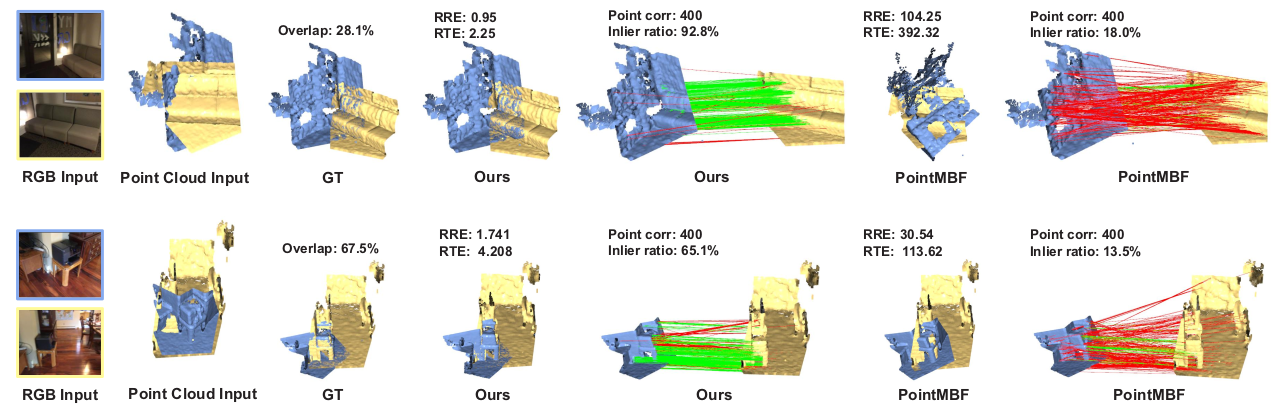
\includegraphics[width=\linewidth]{imgs/3_figure3_in_paper.png}
  \caption{Qualitative comparison with PointMBF.
    \textbf{Row 1}: low-overlap case (28.1\% overlap). OG-UPCR: RRE 0.95°, RTE 2.25;
    inlier ratio 92.8\%. PointMBF: RRE 104.25°, RTE 392.32; inlier ratio 18.0\%.
    \textbf{Row 2}: photometric inconsistency (67.5\% overlap, large viewpoint change).
    OG-UPCR: RRE 1.74°, RTE 4.21; inlier ratio 65.1\%. PointMBF: RRE 30.54°, RTE 113.62;
    inlier ratio 13.5\%. Green lines = correct correspondences; red = outliers.}
  \label{fig:qual}
\end{figure}

\paragraph{OCID inlier ratio (Fig.~\ref{fig:ocid}).}
After applying OCID, correspondences are constrained to the overlapping region, sharply
raising the inlier ratio:
$51.5\% \to \textcolor{OkGreen}{86.5\%}$ (scene 1) and
$48.5\% \to \textcolor{OkGreen}{78.5\%}$ (scene 2).
Red points are outliers; green are inliers.

\begin{figure}[h]
  \centering
  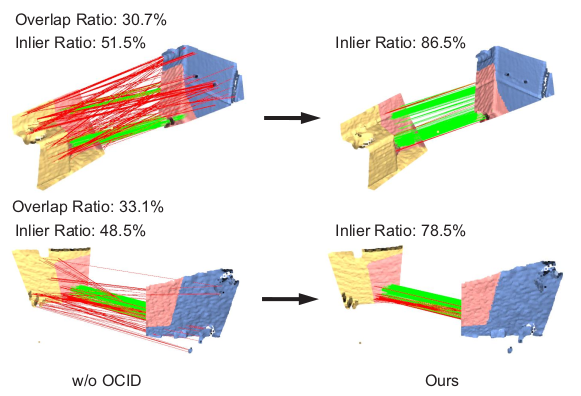
\includegraphics[width=0.82\linewidth]{imgs/4_figure4_in_paper.png}
  \caption{Validation of OCID on inlier detection. Left: without OCID.
    Right: with OCID. After OCID, correspondences are confined to the overlapping region
    (pink), significantly raising the inlier ratio.}
  \label{fig:ocid}
\end{figure}

\paragraph{GRPA rendering quality (Fig.~\ref{fig:grpa}).}
Rendered RGB and depth images compared across three conditions: without GRPA,
with GRPA (Ours), and ground truth. With GRPA, rendering artefacts in the red-highlighted
regions are substantially reduced, improving the photometric consistency signal used for
training.

\begin{figure}[h]
  \centering
  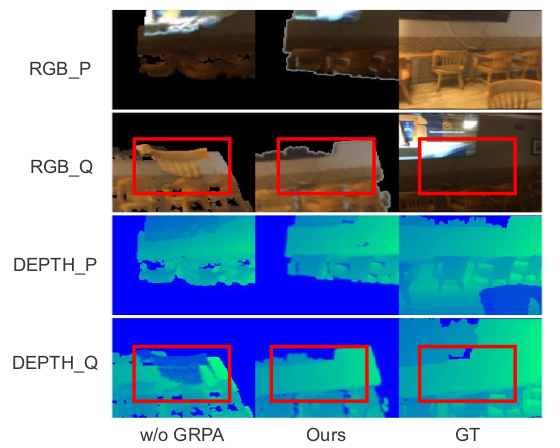
\includegraphics[width=0.82\linewidth]{imgs/5_figure5_in_paper.png}
  \caption{Validation of GRPA for photometric adaptation. Each group shows RGB\_P, RGB\_Q,
    DEPTH\_P, DEPTH\_Q. \textbf{w/o GRPA}: prominent artefacts in red boxes.
    \textbf{Ours}: artefacts significantly reduced. \textbf{GT}: ground-truth reference.}
  \label{fig:grpa}
\end{figure}

%==============================================================
\section{Conclusion}
\label{sec:conclusion}
%==============================================================

OG-UPCR is an unsupervised RGB-D point cloud registration framework specifically designed
for the two most challenging real-world conditions: \emph{low overlap} and \emph{photometric
inconsistency}.

The \textbf{OCID} module addresses low overlap by enforcing a global overlapping constraint
on correspondences. Its two-stage design — random overlapping region prediction for
outlier rejection and global-to-local inlier detection for spatial coverage — reliably
identifies true inlier correspondences without ground-truth poses.

The \textbf{GRPA} module addresses photometric inconsistency by replacing the
nearest-point PyTorch3D rasteriser with 3D Gaussian splatting and learnable per-pixel
photometric adaptation. This allows the photometric consistency loss to remain meaningful
even when the same surface looks different across views.

Trained end-to-end without ground-truth poses, OG-UPCR achieves \textbf{state-of-the-art
unsupervised performance} on 3DMatch and ScanNet. On the hard ScanNet1500 benchmark, it
is \emph{comparable to the supervised BUFFER} — a remarkable result for an unsupervised
method — and significantly surpasses all other unsupervised approaches.

%==============================================================
\section*{Appendix A: Notation Table}
\label{sec:appendix}
%==============================================================

For quick reference, this appendix collects the notation used across the OCID
(Sec.~\ref{sec:ocid}) and GRPA (Sec.~\ref{sec:grpa}) formulas.

\subsection*{A.1 General / Input Notation}
\begin{center}
\begin{tabular}{@{}p{0.3\linewidth}p{0.62\linewidth}@{}}
\toprule
Symbol & Meaning \\
\midrule
$P,\ Q$ & The two point clouds (RGB-D frames) to be registered \\
$\mathbf{p}_i,\ \mathbf{q}_j$ & The $i$-th point of $P$, $j$-th point of $Q$ ($\in\mathbb{R}^3$) \\
$N$ & Number of points in $P$ (analogously for $Q$) \\
$F_P^f,\ F_Q^f$ & Fused (2D+3D) descriptors of $P,Q$; $\in\mathbb{R}^{N\times C_{3D}}$ \\
$C_{3D}$ & Feature dimensionality per point \\
$I^P,\ D^P$ & Ground-truth RGB and depth images of frame $P$ (similarly $I^Q,D^Q$) \\
$\odot$ & Rigid transform applied to a point cloud ($\mathbf{T}\odot P$) \\
$[\![\,\cdot\,]\!]$ & Iverson bracket: $1$ if the condition holds, $0$ otherwise \\
\bottomrule
\end{tabular}
\end{center}

\subsection*{A.2 OCID Notation}
\begin{center}
\begin{tabular}{@{}p{0.3\linewidth}p{0.62\linewidth}@{}}
\toprule
Symbol & Meaning \\
\midrule
$D(\cdot,\cdot)$ & L2 distance in \emph{feature} space (not 3D space) \\
$\mathbf{q}_j^{1nn},\ \mathbf{q}_j^{2nn}$ & Nearest and 2nd-nearest feature-space neighbours of $\mathbf{p}_i$ \\
$r_i$ & Lowe's ratio of $\mathbf{p}_i$: $D_{1nn}/D_{2nn}\in(0,1]$; smaller = more confident \\
$w=1-r$ & Soft correspondence confidence weight \\
$k$ & Top-$k$ retained per direction ($P\!\to\!Q$, $Q\!\to\!P$) \\
$C_{\text{initial}}$ & Initial correspondence set, $2k$ triples $(\mathbf{p},\mathbf{q},w)$ \\
\midrule
$C_n$ & Random subset of $C_{\text{initial}}$ sampled in RO (RANSAC-style) \\
$r$ (RO) & Sampling ratio, $r=0.2$; subset size $2rk$ \\
$\mathbf{T}_s$ & Trial transformation estimated from $C_n$ via Weighted SVD \\
$P'=\mathbf{T}_s\odot P$ & $P$ after applying the trial transform \\
$O_p$ & Overlap ratio produced by $\mathbf{T}_s$ \\
$\tau$ & Inlier distance threshold, $\tau=5\,$cm \\
$O_{thr}$ & Threshold classifying a subset as positive/negative \\
$w_r,\ w_p$ & Reward / penalty weight factors; $w_r\cdot w_p=1$ \\
$N$ (RO rounds) & Number of sample-evaluate iterations \\
$k_f$ & Top-$k_f$ retained after RO \\
$C_f,\ w_f$ & Optimised correspondence set and its weights (used in GL and $L_{corr}$) \\
\midrule
$C_{ij}$ & First-order compatibility: $1$ if pair $i,j$ preserves distance ($d_{ij}\le d_{thr}$) \\
$SC^2_{ij}$ & Second-order spatial compatibility \\
$d_{ij}$ & Length-preservation residual $\bigl|\lVert\mathbf{p}_i-\mathbf{p}_j\rVert-\lVert\mathbf{q}_i-\mathbf{q}_j\rVert\bigr|$ \\
$d_{thr}$ & Compatibility distance threshold, $d_{thr}=10\,$cm \\
$R$ & Neighbourhood radius for spatially-spread seed selection \\
seed / $K$ & High-confidence seed point; top-$K$ neighbours form its consensus set \\
$\mathbf{T}_{gs}^0$ & Coarse pose (OCID output), fed into GRPA \\
\bottomrule
\end{tabular}
\end{center}

\subsection*{A.3 GRPA Notation}
\begin{center}
\begin{tabular}{@{}p{0.3\linewidth}p{0.62\linewidth}@{}}
\toprule
Symbol & Meaning \\
\midrule
$\mathbb{G}$ & Set of Gaussians representing a scene ($\mathbb{G}^P,\mathbb{G}^Q$) \\
$\mathbf{x}$ & A 3D query point \\
$g(\mathbf{x})$ & Influence (coverage/alpha) of one Gaussian at $\mathbf{x}$ \\
$\mu_{3D}$ & Gaussian centre (3D point position) \\
$\mathbf{c}$ (or $c_i$) & Gaussian RGB colour $\in\mathbb{R}^3$ \\
$r_{3D}$ (or $r$) & Isotropic radius (plays the role of $\sigma$) \\
$o$ & Opacity $\in[0,1]$ \\
$\Sigma_{3D}$ & Full 3D covariance (general 3DGS; OG-UPCR simplifies to scalar $r_{3D}$) \\
\midrule
$\mu_{2D},\ r_{2D}$ & Projected splat centre and radius on the 2D image \\
$\mathbf{K}$ & Camera intrinsic matrix (focal length $f$, principal point) \\
$\mathbf{T}$ & Camera extrinsic $=[\mathbf{R}\,|\,\mathbf{t}]$ — the pose being refined \\
$\mathbf{T}_0$ & Reference (identity) pose used for cross-rendering \\
$d$ & Depth ($z$ in camera coordinates) \\
$f$ & Focal length \\
$\rho$ & A rendered pixel \\
$g_i(\rho)$ & Value of Gaussian $i$'s influence function at pixel $\rho$ (its alpha) \\
$n$ & Number of Gaussians covering $\rho$, sorted near$\to$far \\
$\prod_{j<i}(1-g_j)$ & Accumulated transmittance from nearer Gaussians \\
$R^{gs}_{rgb},\ R^{gs}_{depth}$ & Rendered colour / depth images (alpha compositing) \\
$\Sigma_{2D},\ \mathbf{J},\ \mathbf{W}$ & Projected 2D covariance; projection Jacobian; view-matrix rotation (EWA) \\
\midrule
$\alpha,\ \beta$ & Per-pixel learnable parameters, re-optimised per frame pair \\
$\exp(\alpha)$ & Gain (always positive) $\to$ corrects contrast/exposure \\
$\beta$ & Bias $\to$ corrects background brightness/ambient level \\
$R^{gs'}_{rgb}$ & Photometrically-adapted render: $\exp(\alpha)R^{gs}_{rgb}+\beta$ \\
\midrule
$L^P_{rgb},\ L^P_{depth}$ & L1 colour / depth loss (render vs.\ ground truth $I^P,D^P$) \\
$L^P_{gs}$ & Total rendering loss for side $P$: $L^P_{rgb}+L^P_{depth}$ \\
$L_{gs}$ & Cross-view rendering loss: $L^P_{gs}+L^Q_{gs}$ \\
$L_{corr}$ & Correspondence consistency loss on $C_f$ \\
$\lambda_{gs},\ \lambda_{corr}$ & Loss balancing weights ($L=\lambda_{gs}L_{gs}+\lambda_{corr}L_{corr}$) \\
$\mathbf{T}_{gs}^R$ & Final pose after GRPA refinement of $\mathbf{T}_{gs}^0$ \\
$\lVert\cdot\rVert_1,\ \lVert\cdot\rVert_2$ & L1 (sum of absolute values) and L2 (Euclidean) norms \\
\bottomrule
\end{tabular}
\end{center}

%==============================================================
\begin{thebibliography}{10}

\bibitem{ravi2020pytorch3d}
N.~Ravi, J.~Reizenstein, D.~Novotny, T.~Gordon, W.-Y.~Lo, J.~Johnson, G.~Gkioxari.
\newblock Accelerating 3D deep learning with {PyTorch3D}.
\newblock \emph{arXiv:2007.08501}, 2020.

\bibitem{lowe2004sift}
D.~G.~Lowe.
\newblock Distinctive image features from scale-invariant keypoints.
\newblock \emph{International Journal of Computer Vision}, 60(2):91--110, 2004.

\bibitem{elbanani2021urr}
M.~El~Banani, L.~Gao, J.~Johnson.
\newblock Unsupervised {R\&R}: Point cloud registration via differentiable rendering.
\newblock In \emph{CVPR}, 2021.

\bibitem{zhang2023pointmbf}
J.~Zhang, R.~Hu, X.~Chen, J.~Gu.
\newblock Point cloud registration with multi-scale bidirectional fusion.
\newblock In \emph{ICCV}, 2023.

\bibitem{kerbl2023gaussiansplatting}
B.~Kerbl, G.~Kopanas, T.~Leimk{\"u}hler, G.~Drettakis.
\newblock {3D} Gaussian splatting for real-time radiance field rendering.
\newblock \emph{ACM TOG}, 2023.

\bibitem{yu2021cofinet}
H.~Yu, F.~Li, M.~Saleh, B.~Busam, S.~Ilic.
\newblock {CoFiNet}: Reliable coarse-to-fine correspondences for robust point cloud registration.
\newblock In \emph{NeurIPS}, 2021.

\bibitem{chen2022sc2pcr}
Z.~Chen, K.~Sun, F.~Yang, W.~Tao, C.~Li.
\newblock {SC2-PCR}: A second order spatial compatibility for efficient and robust point cloud registration.
\newblock In \emph{CVPR}, 2022.

\bibitem{zhang2023mac}
Z.~Zhang, Y.~Sun, Y.~Yao, H.~Shi.
\newblock {MAC}: Maximal cliques for 3D registration.
\newblock In \emph{CVPR}, 2023.

\bibitem{chen2021buffer}
Z.~Chen, K.~Sun, F.~Yang, L.~Guo.
\newblock {BUFFER}: Balancing accuracy, efficiency, and generalizability in point cloud registration.
\newblock In \emph{CVPR}, 2023.

\bibitem{li2019pointnet}
Y.~Li, R.~Bu, M.~Sun, W.~Wu, X.~Di, B.~Chen.
\newblock {RIENet}: Reliable inlier evaluation for unsupervised point cloud registration.
\newblock In \emph{AAAI}, 2022.

\bibitem{qiao2023byoc}
D.~Qiao, F.~Nie, J.~Liu.
\newblock {BYOC}: Bring your own correspondences — unpaired point cloud completion via unsupervised registration.
\newblock In \emph{ICCV}, 2023.

\bibitem{fu2023llt}
K.~Fu, S.~Liu, X.~Luo, M.~Wang.
\newblock {LLT}: Efficient unsupervised point cloud registration for outdoor scenes.
\newblock In \emph{CVPR}, 2023.

\bibitem{qin2022geometric}
H.~Qin, Y.~Shi, H.~Ye.
\newblock {GeoTransformer}: Fast and robust point cloud registration with geometric transformer.
\newblock \emph{TPAMI}, 2023.

\end{thebibliography}

\end{document}
